\begin{frame}{NC 最終調整}
  \centering
  $\pi^+ \pi^-$の運動量を固定して$d(K^-, \pi^+ \pi^-)"X"$が\\ 中性子になるように前方中性子質量を動かす。\\
  調整前
  \tminipageTwo{
    \begin{figure}
      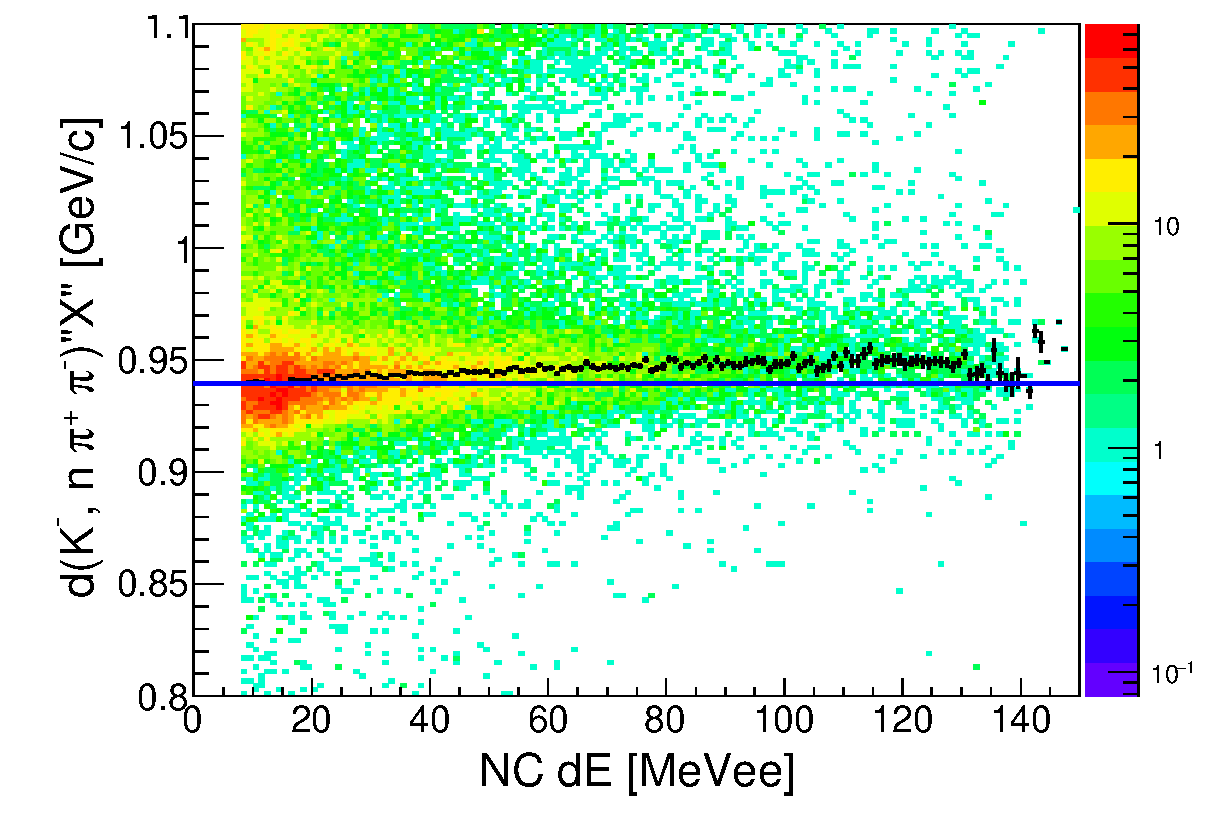
\includegraphics[width=3.5cm]{../pic/Run78/calib/NCdE_KNpipi_MM.eps}
    \end{figure}
  }{
    \begin{figure}
      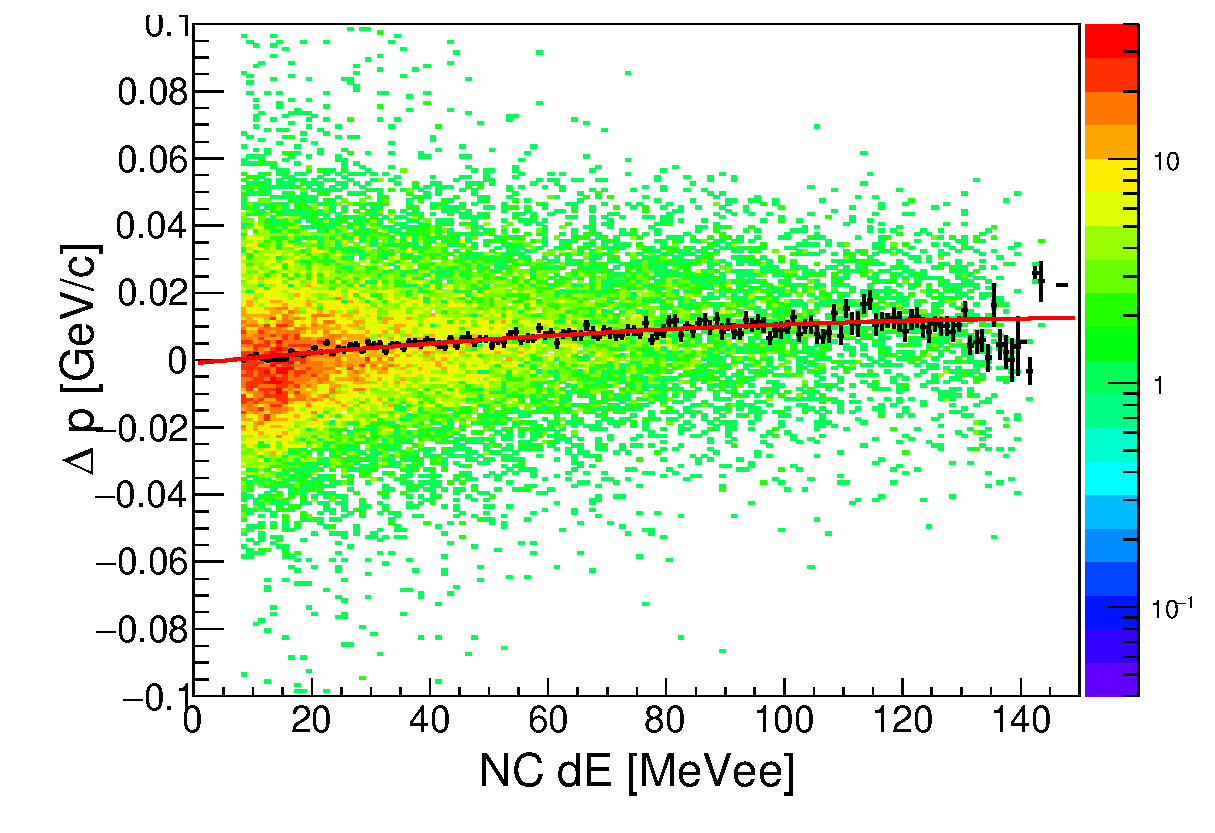
\includegraphics[width=3.5cm]{../pic/Run78/calib/NCdE_delta_p.eps}
    \end{figure}
  }

  調整後
  \tminipageTwo{
    \begin{figure}
      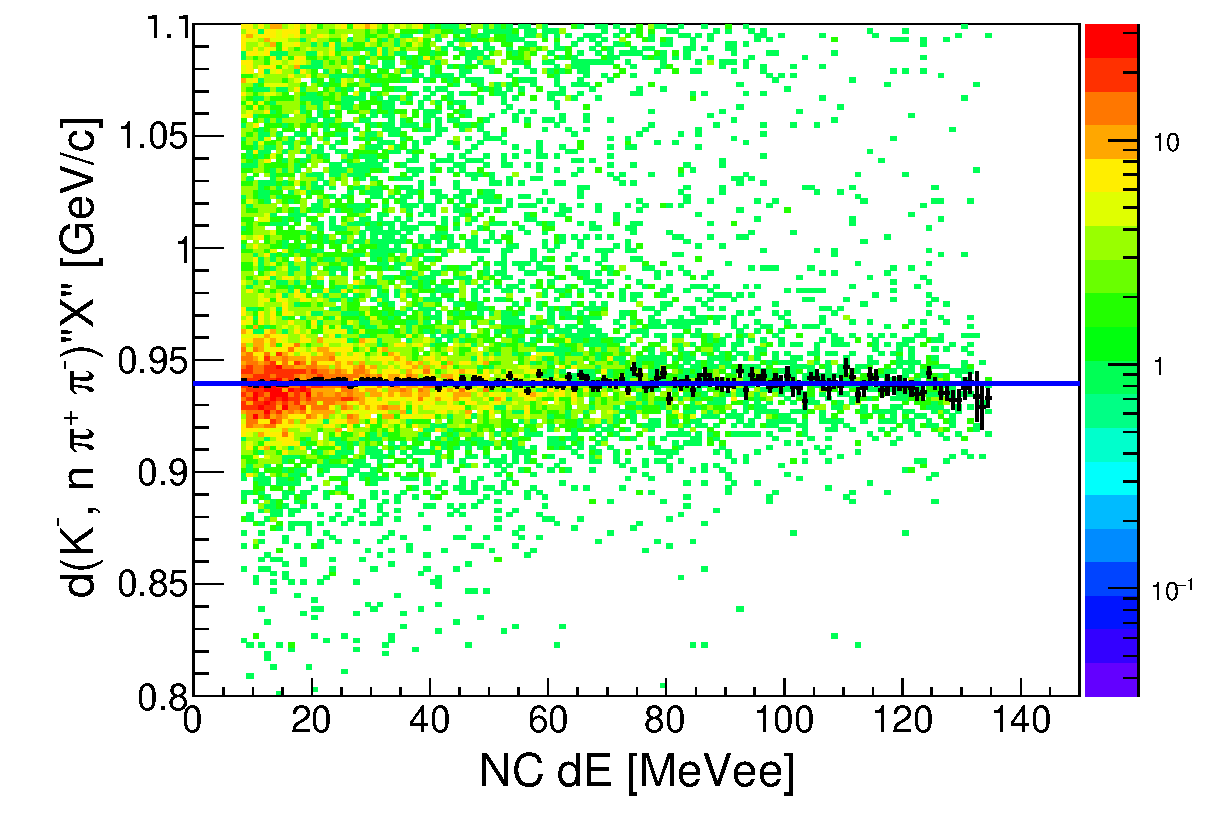
\includegraphics[width=3.5cm]{../pic/Run78/calib/NCdE_KNpipi_MM_mod.eps}
    \end{figure}
  }{
    \begin{figure}
      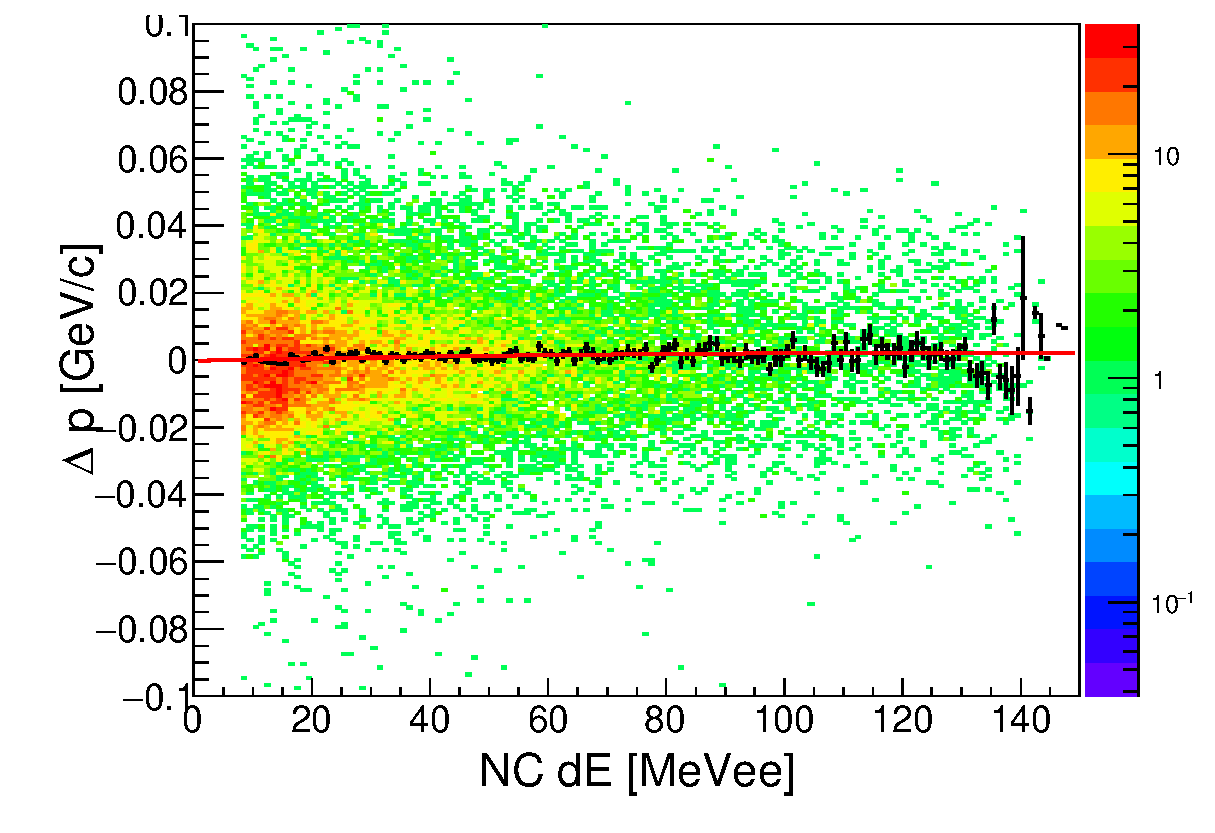
\includegraphics[width=3.5cm]{../pic/Run78/calib/NCdE_delta_p_mod.eps}
    \end{figure}
  }

\end{frame}
